
\runningheader{Oppgave q)}{}{Side \thepage\ av \numpages}


% ********************************************************
% oppgave q) 
% ********************************************************  
  \item[q)]
    I denne oppgaven skal du kun bruke en ferdig modell og ikke
    implementere noe som helst. Hensikten
    er å gi deg litt innsikt i PID-regulatoren som du skal jobbe med i
    det kommende Legoprosjektet.

    PID-regulatoren er den mest brukte regulatoren i industrien, og
    for å forklare virkemåten skal vi benytte en cruisekontroller som
    eksempel og sammenligne med hva som skjer i hjernen vår når vi
    kjører selv, se figur~\ref{fig:neg_feedback3}.
\begin{figure}[H]
  \centering
  \hspace*{5mm}\scalebox{0.38}{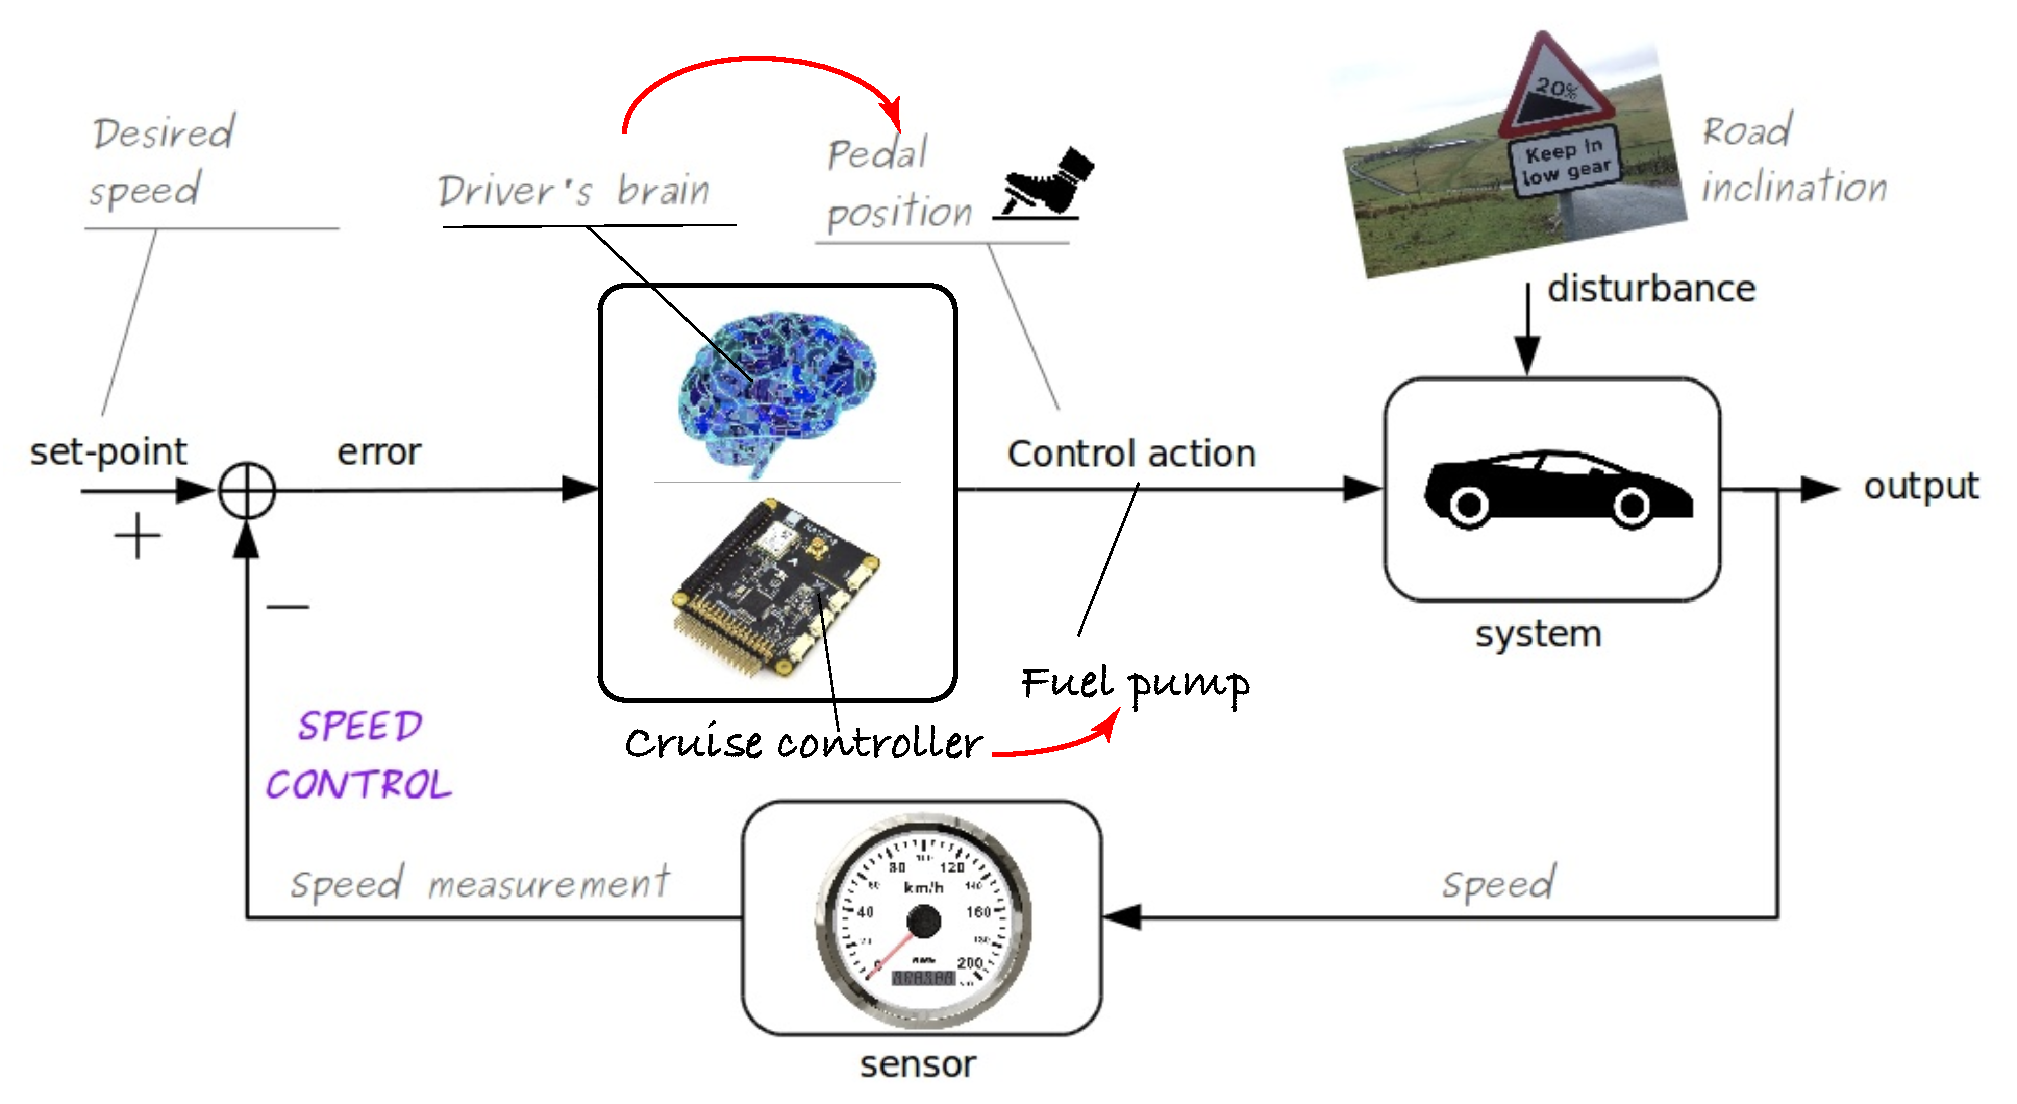
\includegraphics{bil_regulator.pdf}}
  \caption{Prinsippet med negativ tilbakekopling i bilkjøring. Enten
    er det du selv via hjernen din (regulator), øynene dine
    (måleinstrument) og foten din (pådrag) som bestemme farten, eller
    så er det cruisekontrolleren. Hentet fra
    {\color{blue}\href{https://alphaville.github.io/qub/pid-101/}
  {https://alphaville.github.io/qub/pid-101/}}.}
  \label{fig:neg_feedback3}
\end{figure}



Strukturen i figur~\ref{fig:neg_feedback3} kalles
negativ  tilbakekopling, og reguleringssløyfen kan skjematisk
presenteres som i figur~\ref{fig:neg_feedback2}, hvor vi har henviser
til relevante kapitler i kompendiet. 
\begin{figure}[H]
  \centering
  \scalebox{0.55}{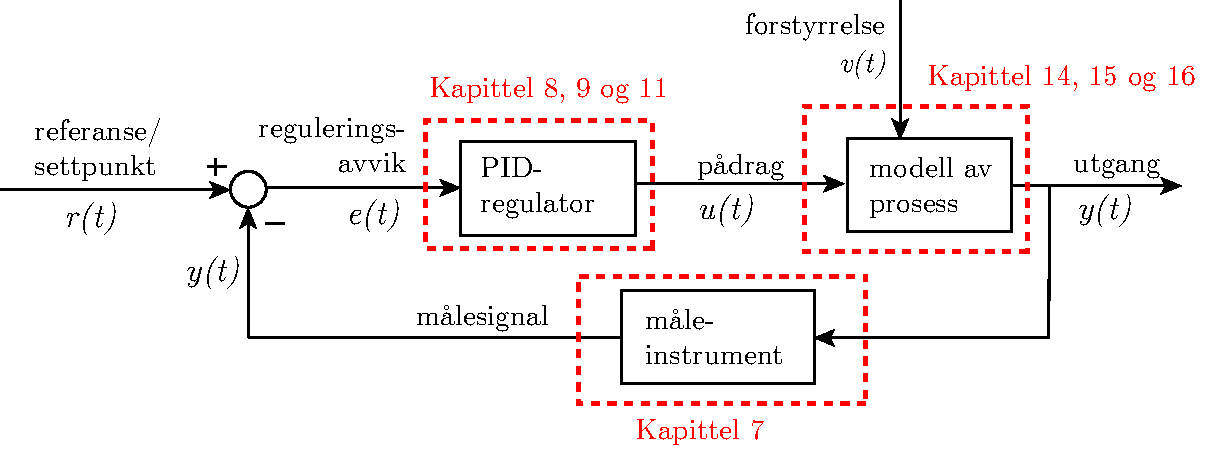
\includegraphics{neg_feedback3.pdf}}
  \caption{Prinsippet for negativ tilbakekopling.}
  \label{fig:neg_feedback2}
\end{figure}
Negativ tilbakekopling innebærer at utgangen $y(t)$ som vi
ønsker å styre/regulere, samples og måles ved hjelp av et
måleinstrument, og dette signalet ``føres tilbake'' og 
sammenlignes med referansen. Siden målingene subtraheres
som markert med minustegnet, oppstår ordet ``negativ''\footnote{Hadde du
  addert $y(t)$ til $r(t)$ ville du 
hatt positiv tilbakekopling.}, og vi 
beregner det såkalte {\it reguleringsavviket} $e(t)$ som
\begin{equation}
  \label{eq:22}
  e(t) = r(t) -y(t)
\end{equation}
Reguleringsavviket er faktisk den eneste informasjonen regulatoren har
tilgang til. {\color{red}Regulatoren har ingen kjennskap til verken
  ønsket verdi $r(t)$ eller utgangens verdi $y(t)$!}
Det betyr at cruisekontrolleren ikke kjenner 
 verken målt fart  eller ønsket fart. Den kjenner kun til 
avviket fra den vilkårlige hastigheten du ønsker å kjøre i.
Poenget er at når avviket $e(t){=}0$, så ``vet'' regulatoren
indirekte at den ukjente målte hastigheten $y(t)$ er lik den ukjente
ønskede hastigheten $r(t)$. En liten kommentar om notasjon:
Strengt tatt er $y(t)$, $r(t)$ og $e(t)$ egentlig diskret verdier gitt
som $\{y_{k}\}$, $\{r_{k}\}$ og $\{e_{k}\}$.


Cruisekontrollen har med andre bare ett mål 
i livet; nemlig å sørge for at $e(t){=}0$ uansett situasjon.
Dette gjelder også
i situasjoner hvor bilen påvirkes av en forstyrrelse~$v(t)$. Tenk på
hva som skjer med hastigheten når du kommer til en
oppoverbakke, som representerer en hindring som reguleringssystemet
ikke har kontroll på. 
Cruisekontrollen oppnår målet i livet sitt ved å beregne et gasspådrag
$u(t)$ som påvirker bilen i en slik retning at målt hastighet $y(t)$
nærmer seg ønsket hastighet $r(t)$, og dermed at $e(t)\rightarrow 0$.
Når du ikke bruker cruisekontroll fungerer du selv som regulator, men
du har jo kontrol på både fart og ønsket fart, men
strengt tatt så gjør du en sammenligning og bruker indirekte avviket
til å enten gi gass eller bremse. 



Matematisk kan PID-regulatoren uttrykkes som ligning~\eqref{eq:10a}, 
hvor ``P'' står for {\it proposjonalvirkning}, ``I'' står
for {\it integralvirkning} og ``D'' står for {\it derivatvirkning}.
\begin{align}
 u(t) = &  \underbrace{K_p{\cdot} e(t)} + 
             \underbrace{\int_0^t K_{i}{\cdot}e(\tau)d\tau} + 
             \underbrace{\frac{d}{dt} \bigr(K_d {\cdot} e(t) \bigl) }   \label{eq:10a}\\
 & \hspace*{13mm} \mathrm{P} \hspace*{18mm} \mathrm{I} 
\hspace*{23mm} \mathrm{D} \notag
\end{align}
hvor $K_p$, $K_{i}$ og $K_{d}$ er forsterkningsfaktorer som kalles
regulatorparametre.
Ligning~\eqref{eq:10a} kan skjematisk
presenteres som figur~\ref{fig:pid_blokk}, hvor P-, I- og
D-delene er representert som tre parallelle bidrag.
\begin{figure}[H]
  \centering
  \hspace*{0mm}\scalebox{0.45}{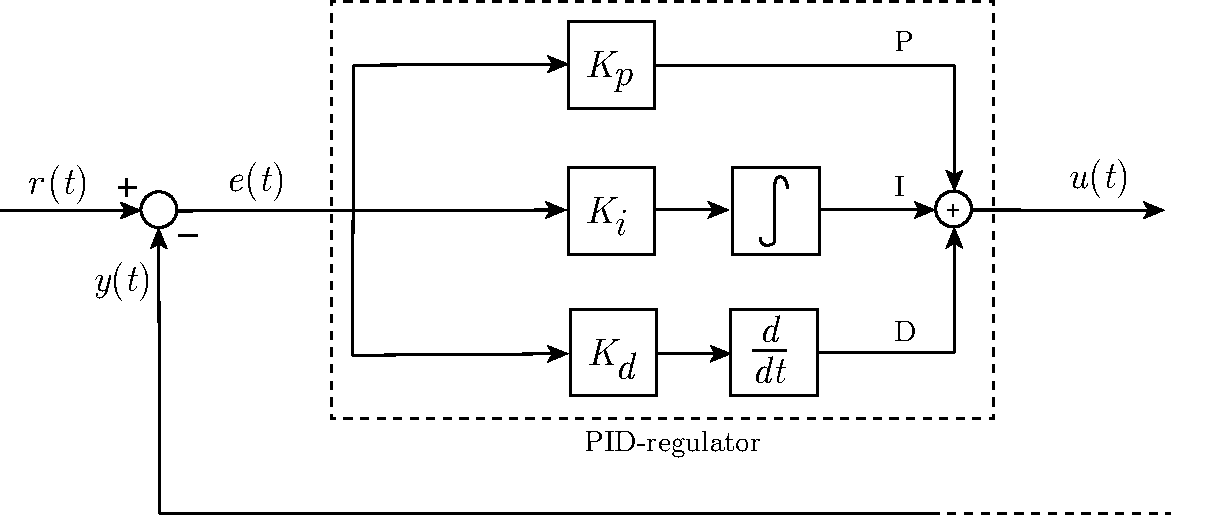
\includegraphics{pid_blokk}}
  \caption{Blokkskjema over  PID-regulatoren i
    ligning~\eqref{eq:10a}.} 
  \label{fig:pid_blokk}
\end{figure}


I simulinkmodellen \fbox{\tt   oving2\_oppg\_q.slx} vist under har 
vi implementert denne PID-strukturen sammen med en
modell av en bil i motbakke.
\begin{figure}[H]
    \centering
    \hspace*{-20mm}\scalebox{0.7}{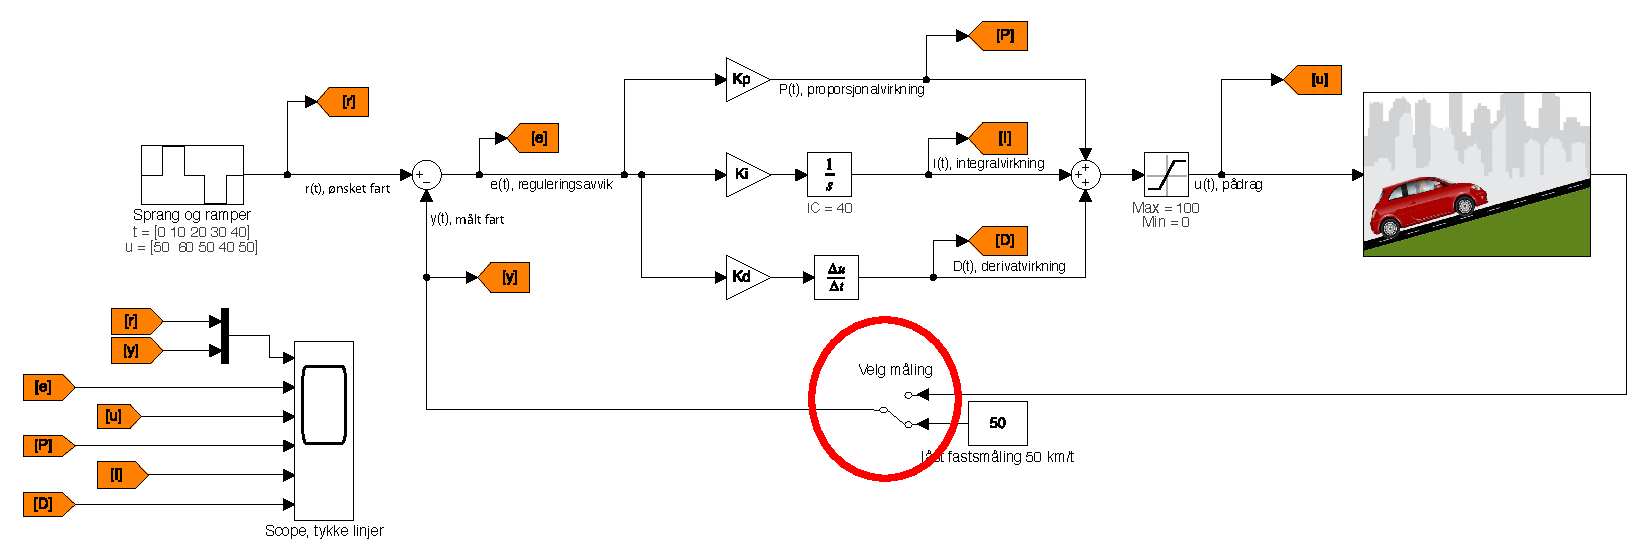
\includegraphics{2q.pdf}}
  \end{figure}
  Situasjonen som er modellert er at bilen kjører i 50~km/t oppover
  en lang bakke, og  pådraget for å oppnå dette er $u(t){=}40$
  (tilsvarer initialverdien til integratoren).
  
Vi har benyttet oss av {\sf  Goto}- og
{\sf   From}-blokker (vist i oransje) slik at modellen blir mindre
spagetti-aktig.  Referansen \fbox{\sf r(t), ønsket fart} helt til venstre
varierer mellom 40 og 60~km/t i løpet av simuleringstiden på 50 sekund.

Den røde ringen markerer en manuell bryter som skifter retning når du
dobbeltklikker på den. Slik bryteren står i figuren antar vi at målt hastighet er
50~km/t uansett hva cruisekontrolleren gjør, og hensikten må å låse
hastigheten er at du skal få anledning til å undersøke hvordan P-, I-,
og D-leddene fungerer før du kopler inn cruisekontrolleren. 

\newpage
    {\bf Gjør følgende oppgaver:    }
    
  \begin{enumerate}[label=q\arabic*)]
  \item  Kjør  filen \fbox{\tt oving2\_data.m}, og simuler modellen og
    bekreft for din egen del at du får responsen i figur~\ref{fig:dump_2q}.
     
  \begin{figure}[H]
    \centering
    \hspace*{10mm}\scalebox{0.7}{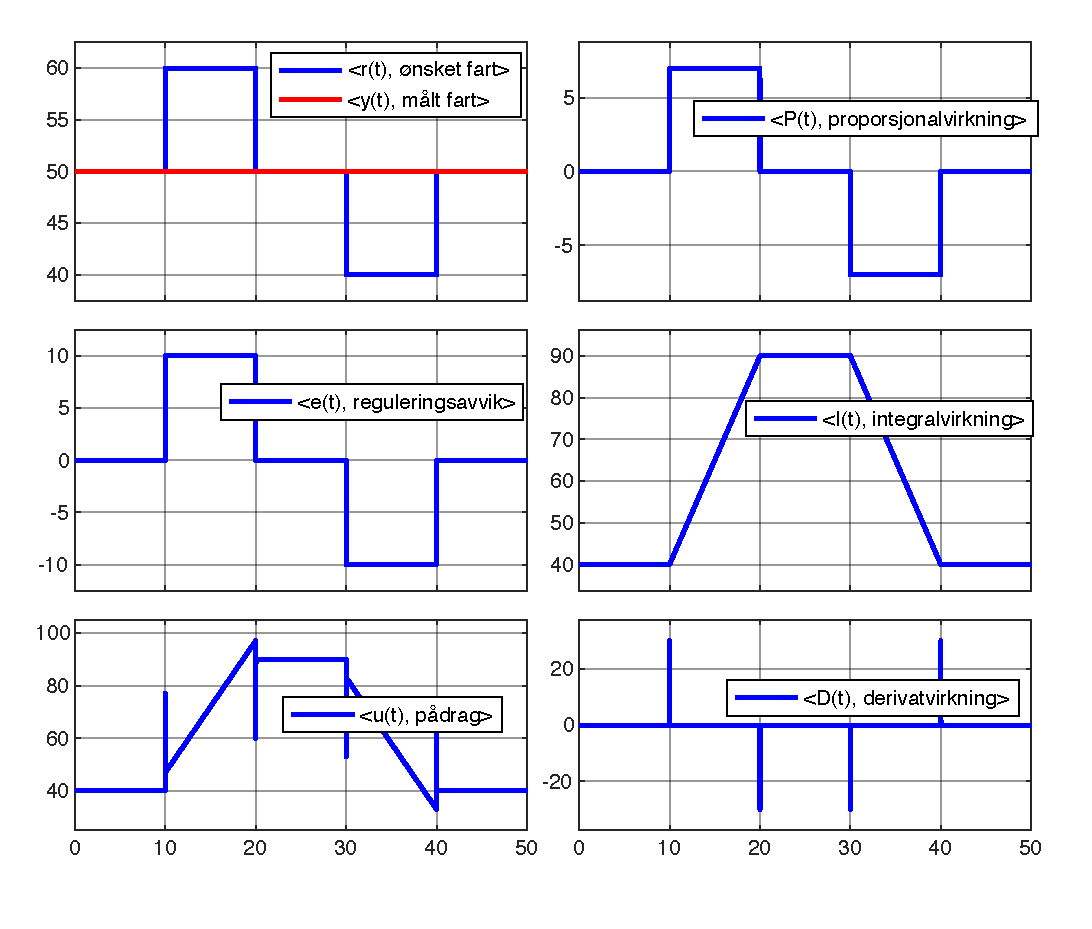
\includegraphics{fig_2q.pdf}}
    \caption{Simuleringsresultat med $K_{p}{=}0.7$, $K_{i}{=}0.5$ og $K_{d}{=}0.03$. }
    \label{fig:dump_2q}
  \end{figure}

  Forklar med dine egne ord hvordan P-, I-, og
  D-leddene fungerer. 

  \item Dobbelklikk på bryteren slik at du måler hastigheten fra
    bilen og at cruisekontrolleren nå er aktiv. Simuler modellen og ta
    med figuren du får i innleveringen. 
    Forklar med ord hva resultatet viser. Fungerer cruisekontrollen
    slik du kjenner den fra din egen erfaring?
  
\item  Endre verdiene av {\sf  Kp}, {\sf  Ki} og
  {\sf  Kd} i m-filen og studere effekten på resultatet. Hvordan
  endres kurvene når regulatorparametrene endres? 
    

 \item Som er frivillig ekstraoppgave kan du prøve å lage din egen
   PID-blokk med din egen meny ved å følge prosedyren i vedlegg~C i kompendiet. 
  
\end{enumerate}




 
